\section{IMAGE Image Display Function}

\subsection{Usage}

The \verb|image| command has the following general syntax
\begin{verbatim}
  handle = image(x,y,C,properties...)
\end{verbatim}
where \verb|x| is a two vector containing the \verb|x| coordinates
of the first and last pixels along a column, and \verb|y| is a
two vector containing the \verb|y| coordinates of the first and
last pixels along a row.  The matrix \verb|C| constitutes the
image data.  It must either be a scalar matrix, in which case
the image is colormapped using the  \verb|colormap| for the current
figure.  If the matrix is \verb|M x N x 3|, then \verb|C| is intepreted
as RGB data, and the image is not colormapped.  The \verb|properties|
argument is a set of \verb|property/value| pairs that affect the
final image.  You can also omit the \verb|x| and \verb|y|, 
\begin{verbatim}
  handle = image(C, properties...)
\end{verbatim}
in which case they default to \verb|x = [1,size(C,2)]| and 
\verb|y = [1,size(C,1)]|.  Finally, you can use the \verb|image| function
with only formal arguments
\begin{verbatim}
  handle = image(properties...)
\end{verbatim}

To support legacy FreeMat code, you can also use the following
form of \verb|image|
\begin{verbatim}
  image(C, zoomfactor)
\end{verbatim}
which is equivalent to \verb|image(C)| with the axes removed so that
the image takes up the full figure window, and the size of the
figure window adjusted to achieve the desired zoom factor using the
\verb|zoom| command.
\subsection{Example}

In this example, we create an image that is \verb|512 x 512| pixels
square, and set the background to a noise pattern.  We set the central
\verb|128 x 256| pixels to be white.
\begin{verbatim}
--> x = rand(512);
--> x((-64:63)+256,(-128:127)+256) = 1.0;
--> figure

ans = 
 1 

--> image(x)
--> colormap(gray)
\end{verbatim}

The resulting image looks like:


\centerline{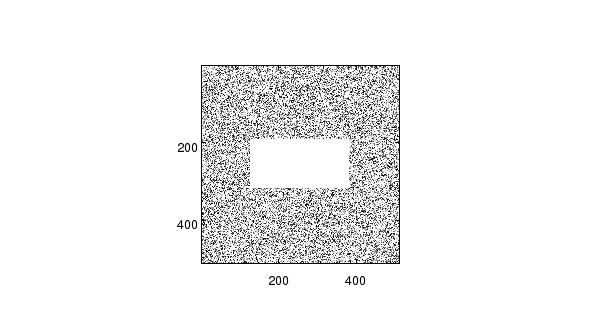
\includegraphics[width=8cm]{image1}}

Here is an example of an RGB image 
\begin{verbatim}
--> t = linspace(0,1);
--> red = t'*t;
--> green = t'*(t.^2);
--> blue = t'*(0*t+1);
--> A(:,:,1) = red; 
--> A(:,:,2) = green; 
--> A(:,:,3) = blue;
--> image(A);
\end{verbatim}
The resulting image looks like:


\centerline{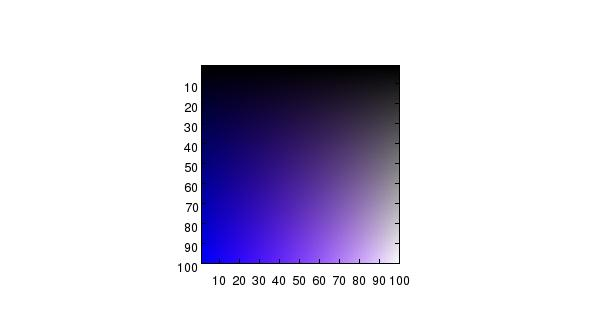
\includegraphics[width=8cm]{image2}}

